%\documentclass[draft]{article}

\documentclass{article}
\usepackage[utf8]{inputenc}
\usepackage[german]{babel}

\setlength{\footskip}{15pt}%Set footer dist.

\usepackage{chemfig}
\usepackage{graphicx}
\graphicspath{ {img/} }
\usepackage{hyperref}
\usepackage{multicol}
\usepackage{amsmath}

\usepackage{fancyvrb}

\usepackage{parskip}%no paragraph indents
\usepackage[landscape, margin=1cm]{geometry}
%\usepackage{adjustbox}

\begin{document}

\begin{multicols*}{3}
%\setlength{\columnseprule}{0.4pt}


\title{Statistik I}
\author{Gian Hiltbrunner}
\maketitle
%Written in \LaTeX{}.

%\noindent\rule{\linewidth}{0.4pt}

\section{Modelle für Zähldaten}
    \subsection{Elementarereignisse}

      Elementarereignisse sind mögliche Ergebnisse oder Ausgänge des Experiments,
      die zusammen den Grundraum bilden:

      $$\Omega =[\sigma]$$

      $\Omega$ = Grundraum: Beinhaltet alle möglichen Elementareregnisse

      $A, B, C,...$ = Ereignisse

      $P$ = Wahrscheinlichkeiten
      \par
      Beispiel: 2-maliges Werfen einer Munze:
      $\Omega = {KK, KZ, ZK, ZZ}$ wobei $K$ = “Kopf” und $Z$ = “Zahl” bezeichnet. Ein
      Elementarereignis ist zum Beispiel $\omega = KZ$.

      \subsubsection{Mengenoperationen}
      $A \cup B \Longleftrightarrow A$ Vereinigung $B$

      $A \cap B \Longleftrightarrow A$ Durchschnitt $B$

      $A \setminus B \Longleftrightarrow A$ ohne $B$

      $A^c \Longleftrightarrow$ nicht $A$

    \subsubsection{Axiome}

      1. Die Wahrscheinlichkeiten sind immer nicht-negativ: P(A) \geq 0

      2. Das Ereignis Ω hat Wahrscheinlichkeit eins: P(\Omega) = 1

      3. P(A∪B) = P(A) + P(B) falls A∩B = \O , d.h. für alle Ereignisse, die sich ¨
      gegenseitig ausschliessen.

      \subparagraph{Weitere Regeln:}

      $$P(A^c) = 1 - P(A) = P(\Omega) - P(A)$$
      $$P(A \cup B) = P(A) + P(B) - P(A \cap B)$$

    \subsection{Laplace-Modell}
      Falls alle Wahrscheinlichkeiten gleich gross sind kann mit dem Laplace-Modell gerechnet werden.
      $$P(E)=\frac{g}{m}$$
      Wobei g: günstige Ereignisse, m: mögliche Ereignisse

    \subsection{Unabhängigkeit}

      Falls  $$ P(A\cap B) = P(A)P(B)$$ gilt, heissen $A$ und $B$ stochastisch unabhängig.

    \subsection{Bedingte Wahrscheinlichkeit}

      $$P(A|B) = \frac{P(A\cap B)}{P(B)}$$
      dabei gilt: $P(A|B) \ne P(B|A)$

      \subsubsection{Gesetz der totalen Wahrscheinlichkeiten}
      $$P(A) = \sum{P(A\cap B_i)} = \sum{P(A|B_i)P(B_i)}$$

      \subsubsection{Satz von Bayes}
      $$P(A|B) = \frac{P(B|A)P(A)}{P(B)}$$
      Dabei kann $P(B)$ im Nenner mit Hilfe des Gesetzes der totalen Wahrscheinlichkeit berechnet werden.

    \subsection{Odds}
      $$ odds(E) = \frac{P(E)}{1-P(E)}$$

      \subsubsection{log-Odds}

      $$log-Odds(E) = \ln (odds(E))$$

      \subsubsection{Odds-Ratio}

      $$ OR = \frac{odds(K|I = 0)}{odds(K|I=1)}$$

    \subsection{Zufallsvariable}

      Eine Zufallsvariable ist ein Zufallsexperiment, das als
      Ergebnis eine Zahl hat.

    \subsection{Bernoulli-Verteilung}

      Benutzt man zur Beschreibung von zufälligen Ereignissen,
      bei denen es nur zwei mögliche Versuchsausgänge gibt.
      Einer der Versuchsausgänge wird meistens mit Erfolg bezeichnet
      und der komplementäre Versuchsausgang mit Misserfolg. (z.B. Münzenwurf)

      $$P(X=1)=\pi, P(X=0)=1-\pi$$

      für $0 \leq \pi \geq 1$.

      $$\operatorname {E}\left(X\right)=p$$

      $${\displaystyle \operatorname {Var} (X)=p\cdot (1-p)=pq}$$
    \subsection{Binominalverteilung}

      Beschreibt die Anzahl der Erfolge in einer Serie von gleichartigen und
      unabhängigen Versuchen, die jeweils genau zwei mögliche Ergebnisse haben
      („Erfolg“ oder „Misserfolg“). Solche Versuchsserien werden auch Bernoulli-Prozesse genannt.
      (vgl. Galton-Brett)
      Eine Zufallsvariable ist binominalverteilt falls,

      $$P(X=x)= \binom{n}{x} \pi ^x (1 - \pi)^{n-x}$$

      Dabei gilt $x = 0,1,...,n$ und $\pi$ ist der Erfolgsparameter.

      \begin{Verbatim}[frame=single]
binomPdf(n,P,{x})
      \end{Verbatim}

      \subsubsection{Approximation durch Normalverteilung}

      Die Binomialverteilung kann durch eine Normalverteilung approximiert werden,
      wenn $n$ hinreichend groß und $p$ weder zu groß noch zu klein ist.
      Als Faustregel dafür gilt $n \pi > 5$ und $n(1 - \pi) > 5$.

      \subsubsection{Kumulative Verteilungsfunktion}

      Die kumulative Verteilungsfunktion ist gegeben als Summe über die Werte der Binominalverteilung von einer unteren zu einer oberen Grenze.
      $$F(x) = P(X\leq x) = \sum_{y\in W_x;y\leq x}{P(X=y)}$$

      \begin{Verbatim}[frame=single]
binomCdf(n, P, Unt. Grenze, Ob. Grenze)
      \end{Verbatim}

    \subsection{Kennzahlen einer Verteilung}
      \subsubsection{Erwartungswert $\epsilon (X)$}
      $$\epsilon (X) = \sum_{x \in W_x}{xP(X=x)}$$

      wobei $W_x$ = Werteberiech von $X$.



      \subsubsection{Varianz}

      Die Varianz beschreibt die erwartete quadratische Abweichung der Zufallsvariablen von ihrem Erwartungswert.

      $$\operatorname {Var}(X):=\operatorname {E}\left((X-\mu )^{2}\right)$$

      \subsubsection{Standardabweichung}
      $$ s = \sqrt{\operatorname {Var}(X)}$$
      $${\displaystyle s={\sqrt {{\frac {1}{n-1}}\sum \limits _{i=1}^{n}\left(x_{i}-{\overline {x}}\right)^{2}}}}$$

      \begin{Verbatim}[frame=single]
stDevSamp({})
      \end{Verbatim}

      Für mehrere Stichproben $\overline{x}=\frac{1}{n}\sum_{i=0}^n{x_n-y_n}$ und $x_i = x_i - y_i$

    \subsection{Verschiedene Verteilungen}

      \subsubsection{Binominalverteilung}
      $$E(X)=np$$
      $$Var(X)=np(1-p)$$
      Falls n gross und $\pi$ klein mit $\lambda = n\pi$.
      \begin{multline}
        $$P(X=x) = \binom{n}{x}\pi^x(1-\pi)^{n-x}\approx P(Y = x) \\ = exp(-\lambda)\frac{\lambda^x}{x!}(x = 0,1,...,n)$$
      \end{multline}

      \subsubsection{Hypergeometrische Verteilung}
      Angenommen, wir haben eine Urne mit N Kugeln. Davon sind m Kugeln markiert
      (= Erfolg) und wir ziehen n Kugeln (ohne Zurucklegen; die Erfolgswahrscheinlichkeit ändert sich also bei jedem Zug) aus der Urne. Die Zufallsvariable
      X beschreibt die Anzahl markierter Kugeln unter den n gezogenen Kugeln.
      Dann gilt X ist hypergeometrisch verteilt: X ∼ Hyper(N, n, m).

      \\$m$: Anzahl der Erfolge in der Population
      \\$N$: Populationsgrösse
      \\$n$: Anzahl an Zügen
      \\$k$: Anzahl der Erfolgszüge

      $$P(X=x)={\frac  {\displaystyle {m \choose k}{N-m \choose n-k}}{\displaystyle {N \choose n}}}$$
      $$E(X)=\frac{nm}{N}$$
      $$Var(X)= \frac{nm(N-m)(N-n)}{N^2(N-1)}$$

      \\Binominalkoeffizient: ${m \choose k}$
      \begin{Verbatim}[frame=single]
nCr(m,k)
      \end{Verbatim}

      \subsubsection{Poisson-Verteilung}
      Der Wertebereich der Binomial$(n, \pi)$-Verteilung ist $W = {0, 1, . . . , n}$. Falls
      eine Zufallsvariable nicht im vornherein einen beschränkten Wertebereich hat, so bietet sich für Zähldaten die Poisson-Verteilung an. z.B. Anzahl Versicherungsfälle pro Jahr.

      $$P_{\lambda }(k)={\frac  {\lambda ^{k}}{k!}}\,{\mathrm  {e}}^{{-\lambda }}$$
      $$E(x)=Var(x)=\lambda$$

      \paragraph{Addition}

      Wenn $X$ $\sim$ Poisson($\lambda *X$) und \\Y $\sim$ Poisson($\lambda *Y$) unabhängig sind, dann gilt \\ $X + Y \sim$ Poisson $(\lambda X + \lambda Y)$.

      \subsubsection{Exponential-Verteilung}
      Anwendungsbeispiele
      \begin{itemize}
        \item Zeit zwischen Anrufen
        \item Lebensdauer von Atomen beim radioaktiven Zerfall
        \item Lebensdauer von Bauteilen, Maschinen und Geräten, wenn Alterungserscheinungen nicht betrachtet werden müssen
        \item Als grobes Modell für kleine und mittlere Schäden in Hausrat, Kraftfahrzeug-Haftpflicht, Kasko in der Versicherungsmathematik
      \end{itemize}
      $\lambda$  steht für die Zahl der erwarteten Ereignisse pro Einheitsintervall.\\

      Dichtefunktion:
      $$f_{{\lambda }}(x)={\begin{cases}\displaystyle \lambda {{\rm {e}}}^{{-\lambda x}}&x\geq 0\\0&x<0\end{cases}}$$
      Die Fläche der Kurve ist auf 1 normiert.
      \\ \\
      Kumulative Verteilungsfunktion:
      $$F(x)=\int \limits _{{0}}^{x}f_{\lambda }\left(t\right)\ {{\rm {d}}}t={\begin{cases}1-{\mathrm  {e}}^{{-\lambda x}}&x\geq 0,\\0&x<0.\end{cases}}$$
      $$E(x)= \frac {1}{\lambda}$$
      $$Var(x)= \frac {1}{\lambda ^2}$$

      \subsubsection{Normalverteilung/Gaussverteilung}

      Die Normal-Verteilung (manchmal auch Gauss-Verteilung genannt) ist die häufigste Verteilung fur Messwerte.\\
      Beispiel: Zufällige Messfehler; Summe von unabhängigen, gleichverteilten Zufallsvariablen \\
      Dichtefunktion:
      $${\displaystyle Y\sim {\mathcal {N}}\left(\mu ,\sigma ^{2}\right)}={\frac {1}{\sqrt {2\pi \sigma ^{2}}}}\operatorname {exp} \left(-{\frac {\left(x-\mu \right)^{2}}{2\sigma ^{2}}}\right)$$
      $$E(x) = \mu$$
      $$Var(x) = \sigma^2$$

      Im Fall $\mu =0$ und $\sigma ^{2}=1$ wird diese Verteilung Standardnormalverteilung genannt. Die Dichtefunktion der Standardnormalverteilung ist
      ${\displaystyle \varphi (x)={\frac {1}{\sqrt {2\pi }}}e^{-{\frac {1}{2}}x^{2}}\,.} {\displaystyle \varphi (x)={\frac {1}{\sqrt {2\pi }}}e^{-{\frac {1}{2}}x^{2}}\,.}$

      \paragraph{Normalisieren}
      $$Z = \frac{X - \mu}{\sigma} \sim N(0, 1)$$

      z.B.: $\frac{Z-4}{2}$ ist normalverteilt nach $N (0, 1)$

\section{Statistik für Zähldaten}
    \subsection{Grundfragen}
    \begin{itemize}
      \item 1. Grundfragestellung: Welches ist der zu den Beobachtungen plausibelste
      Parameterwert? Die Antwort auf diese 1. Grundfrage heisst (Punkt-)Sch¨atzung.
      \item 2. Grundfragestellung: Sind die Beobachtungen kompatibel (statistisch vereinbar)
      mit einem vorgegebenen Parameterwert? Die Antwort auf diese 2. Grundfrage
      heisst statistischer Test.
      \item 3. Grundfragestellung: Welche Parameterwerte sind mit den Beobachtungen
      kompatibel (statistisch vereinbar)? Die Antwort auf diese 3. Grundfrage
      heisst Konfidenzintervall oder Vertrauensintervall. Das Konfidenzintervall
      ist allgemeiner und informativer als ein statistischer Test.
    \end{itemize}

    \subsection{Schätzung für Binominalverteilungen}
    \subsubsection{Momentenmethode}
    Die relative Häufigkeit
    $$\hat{\pi } = \frac{x}{n}$$
    ergibt sich als Schätzung der Erfolgswahrscheinlichkeit.

    \subsubsection{Maximum-Likelihood}
    Ableiten der Wahrscheinlichkeitsfunktion um Maximum zu finden.
    $$\frac{d}{d\pi }{P[X=x]}$$
    Beispiel:\\
    3 Münzwürfe:
    $P(KKZ) = P(K)P(K)P(Z) = p^2(1-p)=p^2-p^3$ $\rightarrow$ Ableiten, null setzen und nach $p$ auflösen.

    \subsection{Statistischer Test}
    \textbf{Null-Hypothese kann nur falsifiziert und nicht verifiziert werden.}
    \begin{itemize}
      \item 1. Modell: $X$: Anzahl Treffer bei $n$ Versuchen;
            $$X \sim Binomial(n, \pi)$$
      \item 2. Spezifiziere die sogenannte Nullhypothese $H_0$:
            $$H_0 : \pi = \pi _0$$
            und (anhand der Problemstellung) eine sogenannte Alternative $H_A$:
            $$H_A : \pi \neq \pi _0$$ (zwei-seitig)
            $$\pi > \pi _0$$ (ein-seitig nach oben)
            $$\pi < \pi _0$$ (ein-seitig nach unten)
            \bigbreak
            Am häufigsten ist die Nullhypothese $H_0 : \pi = 1/2 ($d.h. $ \pi _0 = 1/2)$, also
            ”reiner Zufall” oder ”kein Effekt”. Meist fuhrt man einen Test durch, weil
            man glaubt, dass die Alternative richtig ist und man auch Skeptiker davon
            uberzeugen möchte.
      \item 3. Teststatistik: $T$: Anzahl Treffer bei $n$ Versuchen.
            Verteilung der Teststatistik unter: $$H_0: T \sim Bin(n, \pi _0)^3$$
      \item 4. Lege das sogenannte Signifikanzniveau $\alpha$ fest. Typischerweise wählt
            man $\alpha = 0.05$ (5$\%$) oder auch $\alpha = 0.01$ (1$\%$).
      \item 5. Bestimme den sogenannten Verwerfungsbereich K fur die Teststatistik. Qualitativ zeigt K in Richtung der Alternative:
                \bigbreak
                $K = [0, c_u] \cup [c_o, n]$ falls $H_A : \pi \neq π _0$\bigbreak
                $K = [c, n]$ falls $H_A : \pi > \pi _0$\bigbreak
                ${K = [0, c]}$ falls $H_A : \pi < \pi _0$\bigbreak
                Quantitativ wird K so berechnet, dass $$P_{H_0}(X \in K) = P_\pi _0 (X \in K) \overset{\approx }{\leq } \alpha$$
                Dabei bedeutet $\overset{\approx }{\leq }$, dass die linke Seite kleiner oder gleich der rechten Seite
                sein soll, aber so nahe wie möglich.
      \item 6. Testentscheid: Erst jetzt betrachte, ob der beobachtete Wert der Teststatistik
                in den Verwerfungsbereich $K$ fällt:
                Falls ja: so verwerfe $H_0$ ($H_0$ ist dann statistisch widerlegt, die Abweichung
                von der Nullhypothese ist “signifikant”)
                Falls nein: belasse $H_0$ (was nicht heisst, dass deswegen $H_0$ statistisch bewiesen
                ist).
                Diese Art der Test-Entscheidung beruht auf dem Widerspruchs-Prinzip:
                Hypothesen können nur falsifiziert und nicht verifiziert werden.
    \end{itemize}

    \subsection{Fehler 1. und 2 Art}
    Bei einem statistischen Test treten 2 Arten von Fehlern auf:
    \begin{itemize}
      \item Fehler 1. Art: Fälschliches Verwerfen von $H_0$, obwohl $H_0$ richtig ist.
      \item Fehler 2. Art: Fälschliches Beibehalten von $H_0$, obwohl die Alternative zutrifft.
    \end{itemize}

    \begin{center}
      \begin{tabular}{ l | c | r }
        \hline
         & Wahr $H_0$ & Wahr $H_1$ \\ \hline
        stat. Test $H_0$ & richtig 1-\alpha & Fehler 2.Art \beta \\ \hline
        stat. Test $H_1$ & Fehler 1. Art \alpha & richtig (Macht) 1-\beta \\
        \hline
      \end{tabular}
    \end{center}

    Macht = $1 - P($Fehler 2. Art$) = P($Verwerfen von $H_0$ falls $H_A$ stimmt$) = P_{H_A}(X \in K)$\\
    $P($Fehler 2. Art$) = P ($Beibehalten von $H_0$ falls $H_A$ stimmt)\\
    \bigbreak

    \subsection{Einseitige und zweiseitige Tests}
      \begin{itemize}
        \item Der zweiseitige Test detektiert zwar Abweichungen in beide Richtungen
        von $H_0$, aber die Abweichung muss sehr deutlich sein, damit er sie erkennt.
        $\rightarrow$ Die Macht des zweiseitigen Tests ist klein.
        \item Der einseitige Test detektiert nur Abweichungen in eine Richtung von $H_0$,
        aber die Abweichungen mussen nicht so gross sein, damit er sie erkennt.
        $\rightarrow$ Die Macht des einseitigen Tests ist gross.
      \subsubsection{Beispiel zweiseitiger Test}

      \end{itemize}
        \begin{itemize}
          \item Modell: X: Anzahl Würfe, die Kopf zeigen, wenn man 10 mal wirft. (X \sim Bin(10, $\pi$))
          \item Nullhypothese: $H_0 : \pi = 0.5$, Alternative: $H_A : \pi = 0.5$
          \item Teststatistik: T: Anzahl Wurfe, die Kopf zeigen, wenn man 10 mal wirft.
          Verteilung der Teststatistik unter $H_0: T \sim Bin(10, 0.5)$
          \item  Signifikanzniveau: $\alpha = 0.05$
          \item Verwerfungsbereich: Den zweiseitigen Verwerfungsbereich kann man
          leicht berechnen: Zunächst bestimmt man die Verwerfungsbereiche ($K_>$
          und $K_<$) fur die einseitigen Alternativen $H_A : \pi > 0.5$ und $H_A : \pi <
          0.5$ mit dem halben Signifikanzniveau $\alpha / 2 = 0.025$.
          \item Für das Beispiel gilt also: $$K_2=K_< \cup K_> = \{0,1\} \cup \{9,10\}$$.
          \item Weil ich nicht gesagt habe, wie oft wir Kopf beobachten,
          können wir den Testentscheid nicht fällen.
        \end{itemize}
    \subsection{Approximation des Verwerfungsbereichs}
      Formen: \\
      $K=[0,c_u]\cup [c_0,n]$, falls $H_A:\pi \neq \pi_0$\\
      $K = [c_>,n]$ falls $H_A:\pi > \pi_0$\\
      $K= [0,c_<]$ falls $H_A: \pi < \pi_0$\\
      Normalapproximation für $\alpha = 0.05$:\\
      $c_u = n\pi _0-1.96\sqrt{n\pi_0(1-\pi_0)}$ abrunden\\
      $c_o = n\pi _0+1.96\sqrt{n\pi_0(1-\pi_0)}$ aufrunden\\
      $c_> = n\pi_0+1.96\sqrt{n\pi_0(1-\pi_0)}$ aufrunden\\
      $c_< = n\pi_0-1.96\sqrt{n\pi_0(1-\pi_0)}$ abrunden\\
      Approx. gut falls $n$ gross und $\pi$ nicht nahe bei 0 oder 1.
    \subsection{Verwerfungsbereich}
      Der Verwerfungsbereich umfasst alle 'extremen' (im Sinne der Alternative) Beobachtungen, falls die Nullhypothese wahr ist. Die Wahrscheinlichkeit, dass eine Beobachtung im Verwerfungsbereich beobachtet wird,
      falls die Nullhypothese richtig ist, ist hoechstens 5\% (Signifikanzniveau). Man muss also die kleinste Zahl $k$ finden, sodass $P(X\geq k)\leq 0.05$.
    \subsection{$p$ -Wert}
    \begin{itemize}
      \item Der P-Wert ist definiert als das kleinste Signifikanzniveau,
      bei dem die Nullhypothese $H_0$ (gerade noch) verworfen wird.
      \item Der P-Wert ist die Wahrscheinlichkeit, unter Gültigkeit der Nullhypothese
      das beobachtete Ergebnis oder ein extremeres zu erhalten.\\\\
      $t$: Beobachtete Werte \\
      $T$: Teststatistik \\
      \item Bei rechtsseitigem Test:
      $${\displaystyle p_{\text{rechts}}:=P(T\geq t\mid H_{0})}$$
      \item Bei linksseitigem Test:
      $${\displaystyle p_{\text{links}}:=P(T\leq t\mid H_{0})}$$
      \item Und bei zweiseitigem Test:
      $${\displaystyle p=2\cdot \min\{p_{\text{rechts}},p_{\text{links}}\}}$$
    \end{itemize}

    \subsection{Vertrauensintervall}
    Ein Vertrauensintervall $I$ zum Niveau $1 - \alpha$ besteht aus allen Parameterwerten,
    die im Sinne des statistischen Tests zum Signifikanzniveau $\alpha$ mit der Beobachtung
    verträglich sind.
    $I=\{\pi _0$; Nullhypothese $H_0$ : $\pi = \pi _0$ wird belassen$\}$

    Ein häufig verwendetes Konfidenzniveau ist 95$\% $, so dass in diesem Fall (mindestens) 95 $\%$ aller auf Grundlage von gemessenen Daten berechneten Konfidenzintervalle den wahren Wert der zu untersuchenden Population beinhalten.
    Die häufig anzutreffende Formulierung, dass der wahre Wert mit 95 $\%$ Wahrscheinlichkeit im Konfidenzintervall liegt, d. h. im vorliegenden berechneten Intervall, ist streng genommen nicht korrekt – der wahre Wert liegt entweder in diesem Intervall, oder er liegt nicht darin.

    \begin{figure1}
      \caption{Konfidenzintervalle zum Niveau 95 $\%$ für 100 Stichproben vom Umfang 30
      aus einer normalverteilten Grundgesamtheit. Davon überdecken
      94 Intervalle den exakten Erwartungswert $\mu$ = 5; die übrigen 6 tun das nicht.}
      \centering
      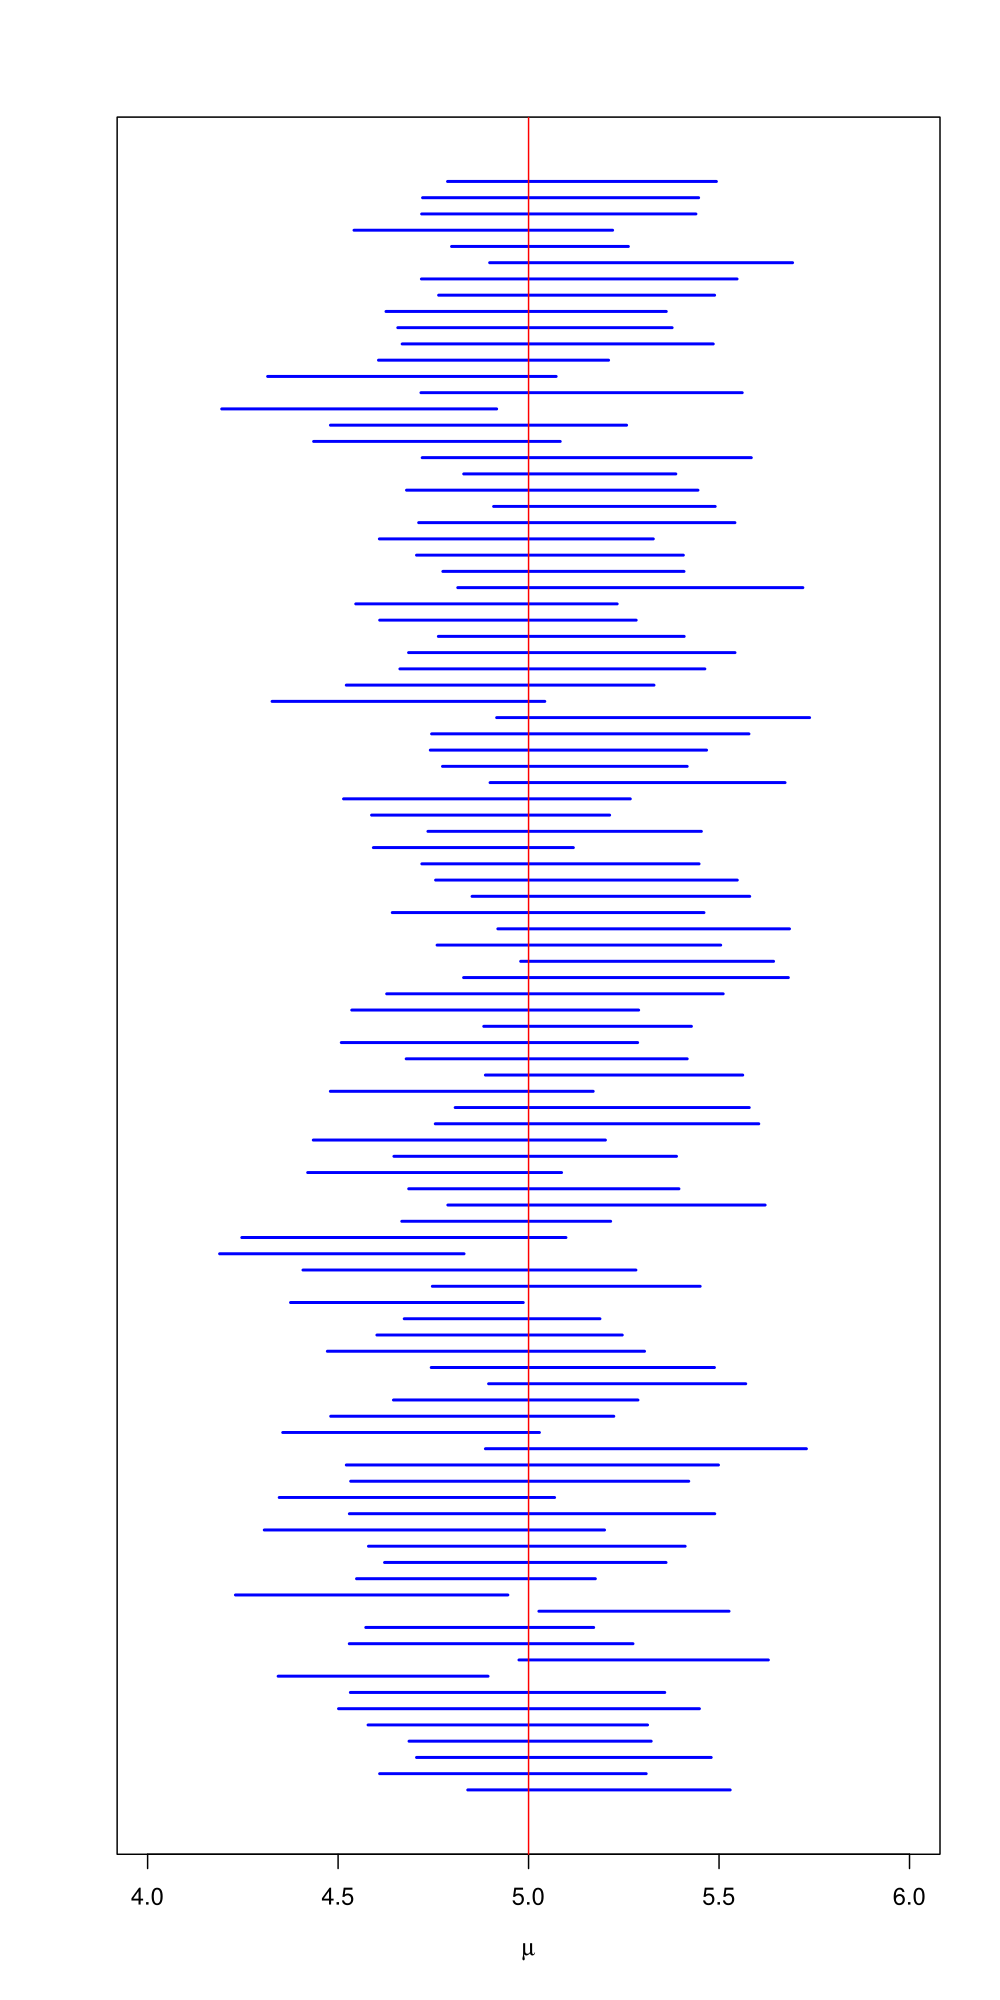
\includegraphics[scale=0.12, angle=90]{coni}
    \end{figure1}

    \subsection{Approximation}

    Für grosse $n$ kann eine Normalapproximation für das $95\%$ Vertrauensintervall verwendet werden.
    $$I \approx \frac{x}{n} \pm 1.96 \sqrt{\frac{x}{n}(1- \frac{x}{n})\frac{1}{n}}$$

\section{Modelle und Statistik für Messdaten}

  \subsection{Kennzahlen}
  Arithmetisches Mittel:
  $${\displaystyle {\overline {x}}={\frac {1}{n}}\sum _{i=1}^{n}{x_{i}}}$$
  Empirische Standardabweichung:
  $${\displaystyle s={\sqrt {{\frac {1}{n-1}}\sum \limits _{i=1}^{n}\left(x_{i}-{\overline {x}}\right)^{2}}}}$$
  \\
  \paragraph{Mittel von unabhängigen, gleichverteilten Messungen}
  Das arithmetische Mittel von $n$ unabhängigen, gleichverteilten Messungen ist zuverlässiger
  als eine Einzelmessung. Genauer gesagt: Die Standardabweichung des arithmetischen Mittels ist um
  den Faktor $\sqrt{n}$ kleiner als die einer Einzelmessung
  $$\sigma _{neu} = \sigma _{alt}/\sqrt{n}$$
  \subsection{Transformationen}

  %Für eine Transformation $g(x) = a + bx (a, b \in R)$ gilt:

  $$Y=a+bX$$
  $$E(Y) = E(a + bX) = a + b E(X)$$
  $$Var(Y) = Var(a + bX) = b^2 Var(X)$$
  $$\sigma Y = |b|\sigma _X$$
  $$\alpha -\text{Quantil}(Y) = q_Y (\alpha) = a + b_{qX}(\alpha)$$

  Negatives Vorzeichen ebenfalls quadrieren!

  \subsection{Zentraler Grenzwertsatz}
  Falls $X_1,...,X_n$ i.i.d.(Unabhängig und identisch verteilt), dann: \\
  $$\overline{X}_n \approx N(\mu, \sigma ^2_X/n)$$
  $$S_n \approx N(\mu n, n\sigma^2_X)$$
  wobei die Approximation im Allgemeinen besser wird mit grösserem n. \\
  Standardisierte Zufallsvariable:
  $$Z_{n}={\frac  {S_{n}-n\mu }{\sigma {\sqrt  {n}}}}$$

  \subsubsection{Quantile}
  Das empirische $\alpha$-Quantil ist anschaulich gesprochen der Wert, bei dem $\alpha *
  100 \%$ der Datenpunkte kleiner und $(1 - \alpha) * 100\%$ der Punkte grösser sind.
  \\Das empirische Quantil beträgt:
  $${\displaystyle x_{p}={\begin{cases}{\tfrac {1}{2}}(x_{n\cdot p}+x_{(n\cdot p)+1}),&{\text{wenn }}n\cdot p{\text{ ganzzahlig,}}\\x_{\lfloor n\cdot p+1\rfloor },&{\text{wenn }}n\cdot p{\text{ nicht ganzzahlig.}}\end{cases}}}$$
  Bemerkung: \textbf{Der Median entspicht gerade dem 50$\%$-Quantil.}
  \\\\ Die Quartilsdifferenz ist gleich:
  \\ \textbf{empirisches 75\%-Quantil - empirisches 25\%-Quantil}
  \\ und ist ein Streuungsmass fur die Daten.

  \subsection{Korrelation und empirische Korrelation}
  \textbf{Korrelation impliziert keinen kausalen Zusammenhang!}
  Kovarianz:
  $$\operatorname {cov}(X,Y):=\operatorname E{\bigl [}(X-\operatorname E(X))\cdot (Y-\operatorname E(Y)){\bigr ]}$$
  Korrelation:
  $$\rho _{X,Y}=\mathrm {corr} (X,Y)={\mathrm {cov} (X,Y) \over \sigma _{X}\sigma _{Y}}={E[(X-\mu _{X})(Y-\mu _{Y})] \over \sigma _{X}\sigma _{Y}}$$
  empirische Korrelation:
  $$r_{xy}={\frac {\sum \limits _{i=1}^{n}(x_{i}-{\bar {x}})(y_{i}-{\bar {y}})}{(n-1)}} $$

  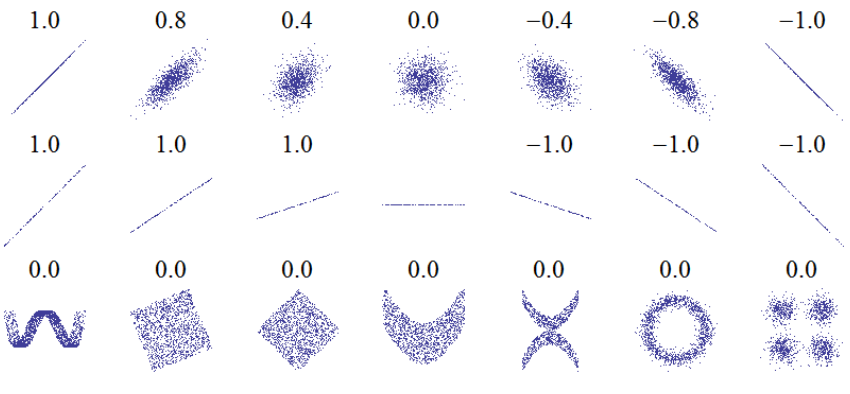
\includegraphics[scale=0.28, angle=0]{korr}

  \subsubsection{Standardisierung}

  Ist $X$ eine Zufallsvariable mit Erwartungswert ${\displaystyle \operatorname {E} (X)=\mu } \operatorname {E}(X)=\mu$  und Varianz
  ${\displaystyle \operatorname {Var} (X)=\sigma ^{2}} \operatorname {Var}(X)=\sigma ^{2}$ (und dementsprechend Standardabweichung $\sigma$ ), so erhält man die zugehörige standardisierte Zufallsvariable durch:
  $${\displaystyle Z={\frac {X-\mu }{\sigma }}}$$

  \subsection{Boxplot}

  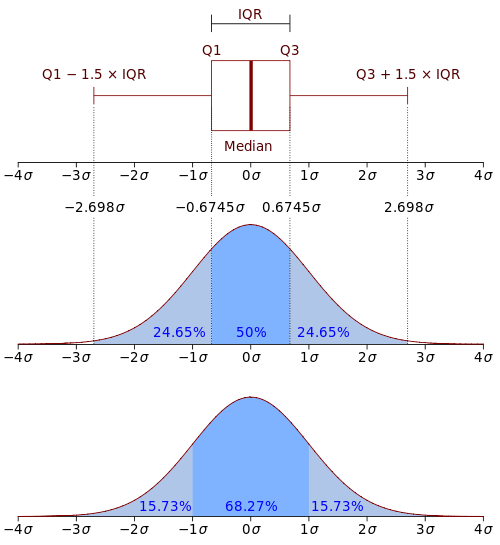
\includegraphics[scale=0.48, angle=0]{box}

  \subsection{Kennzahlen stetiger Verteilungen}
  Dichte
  $$P(x<X\leq x+h) \approx h*f(x)$$
  Erwartungswert
  $$\varepsilon (X) = \int _{-\infty}^{\infty} xf(x)dx$$
  Standardabweichung
  $$Var(X) = \int _{-\infty}^{\infty} (x-\varepsilon(X))^2 f(x)dx$$
  $$\sigma _X = \sqrt{Var(X)}$$

  \subsection{$\sqrt{n}$-Gesetz}
  Die Streuung des arithmetischen Mittels ist nicht proportional zu $\frac{1}{n}$,
  sondern nur zu $\frac{1}{\sqrt{n}}$.

  \subsection{Wichtige stetige Verteilungen}
  vgl. (Verschiedene Verteilungen)\\
    \subsubsection{Uniforme Verteilung}
      \begin{equation}
        f(x)=\begin{cases}
          \frac{1}{b-a}, & \text{falls $a\leq x \leq b$}.\\
          0, & \text{sonst}.
        \end{cases}
      \end{equation}
      Kumulative Verteilungsfunktion:
      \begin{equation}
        f(x)=\begin{cases}
          0, & \text{falls $x<a$}.\\
          \frac{x-a}{b-a}, & \text{falls $ a\leq x \leq b $}.\\
          1, & \text{falls $x > b$}
        \end{cases}
      \end{equation}
      Kennzahlen:\\
      $\Epsilon(X) = \frac{a+b}{2}$\\
      $Var(x)= \frac{(b-a)^2}{12}$

      \subsubsection{Standard-Normalverteilung}

      $$\varphi(x)= \frac{1}{\sqrt{2\pi}} \exp \big\{ -\frac{x^2}{2} \big\}$$
      $$\Phi (x)= \int_{-\infty}^{x}\varphi(x) dy$$

      \subsection{Approximation der t-Verteilung durch Normalverteilung}
      Fur grosse Werte von $n$ ist die Normalverteilung eine ausgezeichnete Approximation
      der $t$-Verteilung. Daher kann man $t_n-2;1-\alpha /2$ mit $\Phi - 1$
      $(1-\alpha /2)$ approximieren.
      Sie sollten sich merken, dass $\Phi-1
      (1 - 0.05/2) = \Phi-1(0.975) ≈ 2$. D.h.,
      eine gute Faustregel fur ein 95\%-Vertrauensintervall ist:
      $$[\beta_0 -2 \text{(s.e)};\beta_0+2\text{(s.e)}]$$
      \subsection{z-Test}
      \subsubsection{Verwerfungsbereich}
      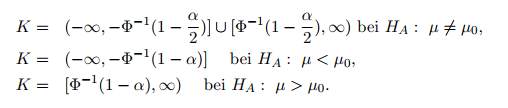
\includegraphics[scale=0.4, angle=0]{z-verwerf}
      \\Tabelle: $df = \infty$

      Normalerweise: $\sigma(t-test) > \sigma(z-test)$
      Für nahe beieinanderliegende Datenpunkte kann es sein, dass
      $\sigma(t-test) < \sigma(z-test)$. Damit wäre dann das Vertrauensintervall des t-Tests kleiner.
      \section{t-Test}

      Die wahre Standardabweichung muss nicht bekannt sein!
      \subsection{Teststatistik für eine Stichprobe}

      $$T=\sqrt{n}*\frac{\overline{X}_n-\mu_0}{\sigma_X}=\sqrt{n}*\frac{D_{vorher-nachher}}{\sigma_X}$$

      \subsubsection{Verwerfungsbereich}
      Zweiseitig:
      $$[-\infty;-t_{n-1;1-\frac{\alpha}{2}}]\cup [t_{n-1;1-\frac{\alpha}{2}};\infty]$$
      Einseitig ($H_A:\mu<\mu_0$) (und vice versa.)
      $$[-\infty;-t_{n-1;1-\alpha}]$$

      \subsubsection{Vertrauensintervall für \mu}
      Zweiseitig:
      $$[\overline{x} _n -t_{n-1,1-\frac{\alpha}{2}} \frac{\hat{\sigma}_X}{\sqrt{n}},\overline{x} _n +t_{n-1,1-\frac{\alpha}{2}} \frac{\hat{\sigma} _X}{\sqrt{n}}]$$
      Einseitig: \\
      Falls $H_A:\mu < \mu _0:$
      $$(-\infty; \overline{x} _n + t_{n-1,1-\alpha} \frac{\hat{\sigma}_X}{\sqrt{n}})$$
      Falls $H_A:\mu < \mu _0:$
      $$(\overline{x} _n - t_{n-1,1-\alpha} \frac{\hat{\sigma}_X}{\sqrt{n}}; \infty)$$

      \subsubsection{Faustregel zu Stichprobengrösse}
      $$n >4*\frac{\sigma^2}{\lambda^2}$$
      $\sigma$: Standardabweichung
      \\$2*\lambda = $ Breite

      \subsubsection{p-Wert}

      Die Anzahl Freiheitsgrade sind $df= n_1 + n_2  - 2 = 20$. Angenommen $T \approx t_{20}$.
      In der Tabelle der t-Verteilung liest man dann ab (Zeile $df=20$): $0.995 \rightarrow 2.845$. D.h.,
      bei einem zweiseitigen Test gehoert zur Teststatistik $t=2.845$ der p-Wert $p=2*0.005=0.01$.

      \subsubsection{Welch-Test}

      $$T={\frac  {{\bar  X}-{\bar  Y}-\omega _{0}}{{\sqrt  {{\frac  {S_{X}^{2}}n}+{\frac  {S_{Y}^{2}}m}}}}}\approx t_{\nu }$$

      Obwohl der Welch-Test speziell für den Fall ${\displaystyle \sigma _{X}\neq \sigma _{Y}}$ entwickelt wurde,
      funktioniert der Test nicht gut, wenn mindestens eine der Verteilungen nicht-normal ist, die Fallzahlen klein und stark unterschiedlich
      $( {\displaystyle n\neq m})$ sind.

      \subsubsection{Mann-Whitney-U Test}
      Falls Daten nicht normalverteilt

      \subsubsection{Übersicht ungepaarte Tests}

      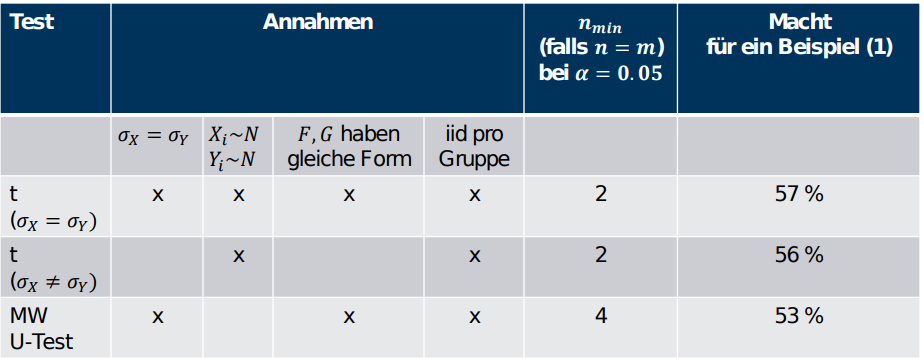
\includegraphics[scale=0.26, angle=0]{stich}

      \subsection{Statistiken für zwei Stichproben}
      \subsubsection{Gepaarte Stichproben}
      $$n= n$$
      \\- beide Versuchsbedingungen an derselben Versuchseinheit eingesetzt werden
      \\- oder jeder Versuchseinheit aus der einen Gruppe genau eine Versuchseinheit
      aus der anderen Gruppe zugeordnet werden kann.

      \\Beispiel:
        Die Wirksamkeit von Augentropfen zur Reduktion des Augeninnendrucks soll
        untersucht werden. Wir haben 12 Patienten. Bei jedem Patienten wählen wir
        zufällig ein Auge aus. In dieses Auge kommen die Augentropfen mit dem Wirkstoff.
        In das andere Auge kommen Tropfen ohne Wirkstoff (Placebo). Fur jede
        Testperson haben wir also zwei Messungen: Eine fur das rechte und eine für
        das linke Auge; die Zuordnung ist eindeutig. Somit handelt es sich um gepaarte
        Stichproben.

      \subsubsection{Ungepaarte Stichproben}

      \\-Beispiel:
        Wir haben die
        Schmelzwärme mit zwei verschiedenen Methoden hintereinander gemessen. Jede
        Messung ist entweder mit Methode A oder mit Methode B, aber nicht mit beiden
        gleichzeitig gemacht worden. Es gibt also keinen eindeutigen Zusammenhang
        zwischen den Messungen der Methode A und den Messungen der Methode B.
        Daher sind die beiden Stichproben ungepaart.

      \subsubsection{Teststatistik für zwei Stichproben}
      $$T = \frac{\overline{X}_n-\overline{Y}_m}{S_{pool}\sqrt{1/n+1/m}}$$
      $\rightarrow$ \textbf{Wurzel ziehen aus gepooltem Wert!}
    \begin{gather}
      $$S^2_{pool} = \frac{1}{n+m-2}\bigg( \sum_{i=1}^{n}(X_i-\overline{X}_n)^2 + \sum_{i=1}^{m}(Y_i-\overline{Y}_m)^2\bigg)
      \\ = \frac{1}{n+m-2}((n-1)\sigma_x^2+((m-1)\sigma_y^2)$$
    \end{gather}
    \subsection{Vorzeichen-Test}
    Die Stichprobenwerte, die größer als der hypothetische Median ${\displaystyle \theta _{0}}$ sind, bekommen ein "$+$" zugeordnet; Werte, die kleiner sind, ein "$-$".
    Das heißt, die Stichprobenvariable wird mediandichotomisiert. Die Anzahl der positiven Vorzeichen wird gezählt und dient als Teststatistik.

    Wir betrachten die Situation, wo die Daten iid. sind, wobei
    die einzelnen $X_i$ nicht normalverteilt sein müssen. Der Vorzeichentest testet Hypothesen über den Median der Verteilung von $X_i$, den wir hier mit $\mu$ bezeichnen;
    im Falle einer symmetrischen Verteilung ist $\mu = E(Xi)$. Wenn $\mu$ der
    Median der Verteilung von $X$ ist, dann ist die Wahrscheinlichkeit, dass eine Realisierung
    von $X$ grösser als $\mu$ ist genauso gross wie die Wahrscheinlichkeit, dass
    eine Realisierung von $X$ kleiner als $\mu$ ist. In anderen Worten: $P(X > \mu) = 0.5$.

    \\Die Nullhypothese des Vorzeichen-Tests lautet $H_0 : \mu = \mu_0$, wobei $\mu$ der Median
    und $\mu_0$ ein vorgegebener, bekannter Wert ist.

    \subsection{Wilcoxon}
    Der Wilcoxon-Test ist ein Kompromiss, der keine Normalverteilung voraussetzt
    wie der t-Test und die Information der Daten besser ausnutzt als der Vorzeichen-Test.
    Die Voraussetzung fur den Wilcoxon-Test ist: Die Daten iid. wobei die Verteilung der $X_i$’s stetig und symmetrisch ist bezuglich $µ =  E(X_i)$

\section{Lineare Regression}
  \subsection{Tabelle lesen}
  \subsubsection{95\% -Vertrauensintervall}
    -Das 95\%-Vertrauensintervall berechnet sich als $(Estimate)\pm c*(Std.Error)$. Für das approximative 95\%-Vertrauensintervall ist c=2.
    \\ -Per Definition enthält das 95\%-Vertrauensintervall alle Parameter $\mu$, bei denen ein Test mit
    der Nullhypothese $H_0 : \beta_0 = \mu$ nicht verwerfen würde.
    \\ -Das 95\%-Vorhersageintervall ist immer breiter als das 95\%- ¨
    Vertrauensintervall für den erwarteten Wert bei gleichen Bedingungen.
  \subsubsection{$p$-Wert}
  Der $p$-Wert kann mit Hilfe des $t$-value aus der Tabelle der $t$-Verteilung mit $n-$(Anzahl geschätzter Koeffizienten)  Freiheitsgraden abgelesen werden.
  \subsubsection{Freiheitsgrade}
  Die Anzahl Freiheitsgrade der $t$-Verteilung berechnet sich aus der Anzahl Datenpunkte ($n$) minus die Anzahl geschätzter Koeffizienten (Anzahl $\beta$)
  \subsubsection{$t$-Wert}
  Der Quotient aus Estimate und Std.Error ergibt den $t$-Wert.
  $$\frac{(Estimate)}{(Std.Error)}=t-Wert$$
  Ist der Wert signifikant auf dem x\%-Niveau?\\
  $\rightarrow$ t-Tabelle
  \subsubsection{Linearität}
  Das Beiwort „linear“ ergibt sich dadurch,
  dass die abhängige Variable eine Linearkombination
  der Regressionskoeffizienten darstellt (aber nicht notwendigerweise der unabhängigen Variablen)
  \\$\beta$s linear!

  \subsection{Vorhersageintervall}
  Das Vorhersageintervall beschreibt den Bereich, in welchem sich der \textbf{wahre Ertrag} für
  gewisse Bedingungen mit $x \%$ Wahrscheinlichkeit befindet.

  \section{QQ-Plots}

  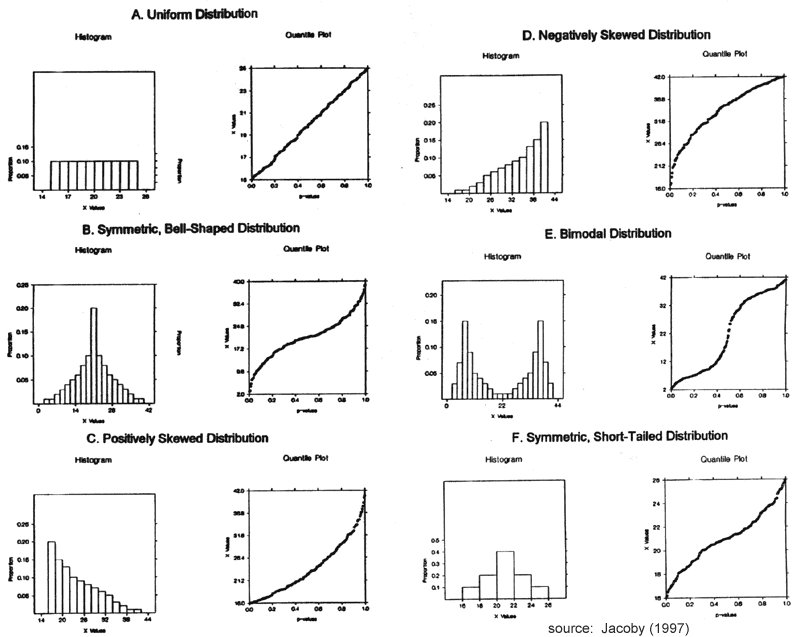
\includegraphics[scale=0.28, angle=0]{qqplots}

  \section{Schiefe}

  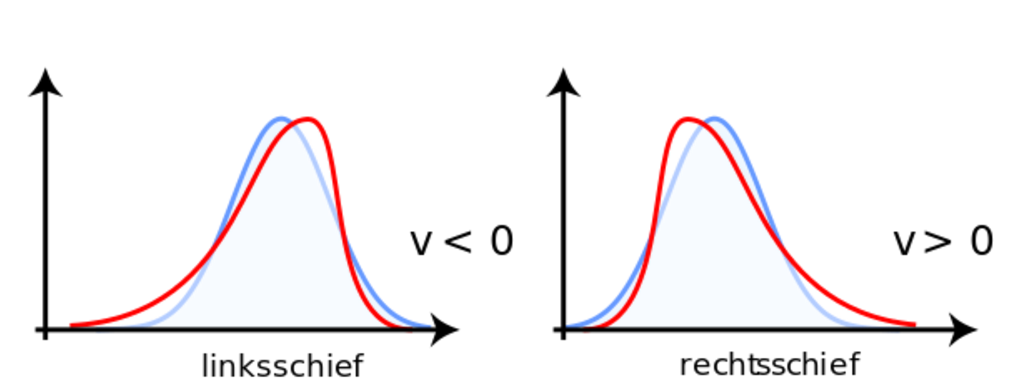
\includegraphics[scale=0.20, angle=0]{lrschief}

  \section{Beispiele}


  \paragraph{Wahrscheinlichkeiten}
  \\$B$ = Frau hat Brustkrebs
  \\$Bc$ = Frau hat keinen Brustkrebs
  \\$Pos$ = positives Testresultat
  \\$Neg$ = negatives Testresultat.
  Gesucht ist $P(B|Pos) = P (Pos|B)*P(B)/P(Pos)$, wobei wir den Satz von Bayes angewendet haben. Die
  Wahrscheinlichkeit ein positives Testresultat zu erhalten berechnet sich als $P(Pos) = P(Pos|Bc)P(Bc)+P(Pos|B)P(B) = (1-P(Neg|Bc))P(Bc)+P(Pos|B)P(B) = (1-0.8)∗0.98+ 0.9∗0.02 = 0.214$
  Deshalb ist $P(B|P os) = 0.9*0.02/0.214 ≈ 0.084$
  \paragraph{Zentraler Grenwertsatz}
  Ein durchschnittlicher Lachsfisch wird etwa 1 m lang und erreicht ein Gewicht von
  10 kg ($\pm$ 2 kg Standardabweichung). Ein Fischerboot fängt an einem guten Tag
  30 Lachsfische. Die Gewichte der Fische seien unabhängig voneinander. Dann ist
  die Wahrscheinlichkeit, dass der Fang mehr als 330 kg wiegt, kleiner als 1\%.

  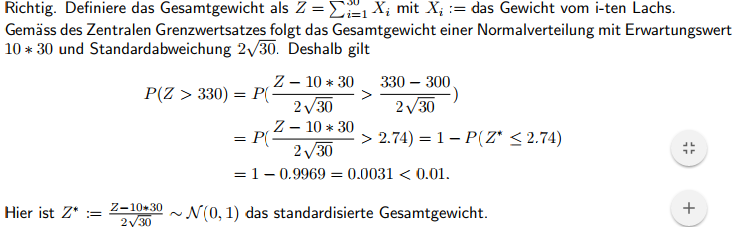
\includegraphics[scale=0.40, angle=0]{a1}


\end{document}
